% Options for packages loaded elsewhere
\PassOptionsToPackage{unicode}{hyperref}
\PassOptionsToPackage{hyphens}{url}
%
\documentclass[
]{article}
\usepackage{amsmath,amssymb}
\usepackage{iftex}
\ifPDFTeX
  \usepackage[T1]{fontenc}
  \usepackage[utf8]{inputenc}
  \usepackage{textcomp} % provide euro and other symbols
\else % if luatex or xetex
  \usepackage{unicode-math} % this also loads fontspec
  \defaultfontfeatures{Scale=MatchLowercase}
  \defaultfontfeatures[\rmfamily]{Ligatures=TeX,Scale=1}
\fi
\usepackage{lmodern}
\ifPDFTeX\else
  % xetex/luatex font selection
\fi
% Use upquote if available, for straight quotes in verbatim environments
\IfFileExists{upquote.sty}{\usepackage{upquote}}{}
\IfFileExists{microtype.sty}{% use microtype if available
  \usepackage[]{microtype}
  \UseMicrotypeSet[protrusion]{basicmath} % disable protrusion for tt fonts
}{}
\makeatletter
\@ifundefined{KOMAClassName}{% if non-KOMA class
  \IfFileExists{parskip.sty}{%
    \usepackage{parskip}
  }{% else
    \setlength{\parindent}{0pt}
    \setlength{\parskip}{6pt plus 2pt minus 1pt}}
}{% if KOMA class
  \KOMAoptions{parskip=half}}
\makeatother
\usepackage{xcolor}
\usepackage[margin=1in]{geometry}
\usepackage{color}
\usepackage{fancyvrb}
\newcommand{\VerbBar}{|}
\newcommand{\VERB}{\Verb[commandchars=\\\{\}]}
\DefineVerbatimEnvironment{Highlighting}{Verbatim}{commandchars=\\\{\}}
% Add ',fontsize=\small' for more characters per line
\usepackage{framed}
\definecolor{shadecolor}{RGB}{248,248,248}
\newenvironment{Shaded}{\begin{snugshade}}{\end{snugshade}}
\newcommand{\AlertTok}[1]{\textcolor[rgb]{0.94,0.16,0.16}{#1}}
\newcommand{\AnnotationTok}[1]{\textcolor[rgb]{0.56,0.35,0.01}{\textbf{\textit{#1}}}}
\newcommand{\AttributeTok}[1]{\textcolor[rgb]{0.13,0.29,0.53}{#1}}
\newcommand{\BaseNTok}[1]{\textcolor[rgb]{0.00,0.00,0.81}{#1}}
\newcommand{\BuiltInTok}[1]{#1}
\newcommand{\CharTok}[1]{\textcolor[rgb]{0.31,0.60,0.02}{#1}}
\newcommand{\CommentTok}[1]{\textcolor[rgb]{0.56,0.35,0.01}{\textit{#1}}}
\newcommand{\CommentVarTok}[1]{\textcolor[rgb]{0.56,0.35,0.01}{\textbf{\textit{#1}}}}
\newcommand{\ConstantTok}[1]{\textcolor[rgb]{0.56,0.35,0.01}{#1}}
\newcommand{\ControlFlowTok}[1]{\textcolor[rgb]{0.13,0.29,0.53}{\textbf{#1}}}
\newcommand{\DataTypeTok}[1]{\textcolor[rgb]{0.13,0.29,0.53}{#1}}
\newcommand{\DecValTok}[1]{\textcolor[rgb]{0.00,0.00,0.81}{#1}}
\newcommand{\DocumentationTok}[1]{\textcolor[rgb]{0.56,0.35,0.01}{\textbf{\textit{#1}}}}
\newcommand{\ErrorTok}[1]{\textcolor[rgb]{0.64,0.00,0.00}{\textbf{#1}}}
\newcommand{\ExtensionTok}[1]{#1}
\newcommand{\FloatTok}[1]{\textcolor[rgb]{0.00,0.00,0.81}{#1}}
\newcommand{\FunctionTok}[1]{\textcolor[rgb]{0.13,0.29,0.53}{\textbf{#1}}}
\newcommand{\ImportTok}[1]{#1}
\newcommand{\InformationTok}[1]{\textcolor[rgb]{0.56,0.35,0.01}{\textbf{\textit{#1}}}}
\newcommand{\KeywordTok}[1]{\textcolor[rgb]{0.13,0.29,0.53}{\textbf{#1}}}
\newcommand{\NormalTok}[1]{#1}
\newcommand{\OperatorTok}[1]{\textcolor[rgb]{0.81,0.36,0.00}{\textbf{#1}}}
\newcommand{\OtherTok}[1]{\textcolor[rgb]{0.56,0.35,0.01}{#1}}
\newcommand{\PreprocessorTok}[1]{\textcolor[rgb]{0.56,0.35,0.01}{\textit{#1}}}
\newcommand{\RegionMarkerTok}[1]{#1}
\newcommand{\SpecialCharTok}[1]{\textcolor[rgb]{0.81,0.36,0.00}{\textbf{#1}}}
\newcommand{\SpecialStringTok}[1]{\textcolor[rgb]{0.31,0.60,0.02}{#1}}
\newcommand{\StringTok}[1]{\textcolor[rgb]{0.31,0.60,0.02}{#1}}
\newcommand{\VariableTok}[1]{\textcolor[rgb]{0.00,0.00,0.00}{#1}}
\newcommand{\VerbatimStringTok}[1]{\textcolor[rgb]{0.31,0.60,0.02}{#1}}
\newcommand{\WarningTok}[1]{\textcolor[rgb]{0.56,0.35,0.01}{\textbf{\textit{#1}}}}
\usepackage{longtable,booktabs,array}
\usepackage{calc} % for calculating minipage widths
% Correct order of tables after \paragraph or \subparagraph
\usepackage{etoolbox}
\makeatletter
\patchcmd\longtable{\par}{\if@noskipsec\mbox{}\fi\par}{}{}
\makeatother
% Allow footnotes in longtable head/foot
\IfFileExists{footnotehyper.sty}{\usepackage{footnotehyper}}{\usepackage{footnote}}
\makesavenoteenv{longtable}
\usepackage{graphicx}
\makeatletter
\def\maxwidth{\ifdim\Gin@nat@width>\linewidth\linewidth\else\Gin@nat@width\fi}
\def\maxheight{\ifdim\Gin@nat@height>\textheight\textheight\else\Gin@nat@height\fi}
\makeatother
% Scale images if necessary, so that they will not overflow the page
% margins by default, and it is still possible to overwrite the defaults
% using explicit options in \includegraphics[width, height, ...]{}
\setkeys{Gin}{width=\maxwidth,height=\maxheight,keepaspectratio}
% Set default figure placement to htbp
\makeatletter
\def\fps@figure{htbp}
\makeatother
\setlength{\emergencystretch}{3em} % prevent overfull lines
\providecommand{\tightlist}{%
  \setlength{\itemsep}{0pt}\setlength{\parskip}{0pt}}
\setcounter{secnumdepth}{-\maxdimen} % remove section numbering
\ifLuaTeX
  \usepackage{selnolig}  % disable illegal ligatures
\fi
\IfFileExists{bookmark.sty}{\usepackage{bookmark}}{\usepackage{hyperref}}
\IfFileExists{xurl.sty}{\usepackage{xurl}}{} % add URL line breaks if available
\urlstyle{same}
\hypersetup{
  pdftitle={MA 331 Final},
  pdfauthor={Amane Chibana and Harry Wang},
  hidelinks,
  pdfcreator={LaTeX via pandoc}}

\title{MA 331 Final}
\author{Amane Chibana and Harry Wang}
\date{2024-05-06}

\begin{document}
\maketitle

\hypertarget{problem-1}{%
\subsubsection{Problem 1}\label{problem-1}}

\begin{Shaded}
\begin{Highlighting}[]
\NormalTok{pabmi }\OtherTok{=} \FunctionTok{read\_xls}\NormalTok{(}\StringTok{"./pabmi.xls"}\NormalTok{)}

\FunctionTok{with}\NormalTok{(pabmi,}\FunctionTok{cor}\NormalTok{(PA,BMI))}
\end{Highlighting}
\end{Shaded}

\begin{verbatim}
## [1] -0.3854091
\end{verbatim}

\begin{Shaded}
\begin{Highlighting}[]
\FunctionTok{with}\NormalTok{(pabmi,}\FunctionTok{cor.test}\NormalTok{(PA,BMI))}
\end{Highlighting}
\end{Shaded}

\begin{verbatim}
## 
##  Pearson's product-moment correlation
## 
## data:  PA and BMI
## t = -4.1348, df = 98, p-value = 7.503e-05
## alternative hypothesis: true correlation is not equal to 0
## 95 percent confidence interval:
##  -0.5408817 -0.2044696
## sample estimates:
##        cor 
## -0.3854091
\end{verbatim}

The p-value for testing the null hypothesis \(H_0: p(X,Y) = 0\) is
7.503e-05 , which is less than the significance level \(\alpha = 0.05\).
This result allows us to reject the null hypothesis, indicating that the
correlation between PA and BMI is statistically significant and not
zero.

\hypertarget{problem-2}{%
\subsubsection{Problem 2}\label{problem-2}}

\begin{Shaded}
\begin{Highlighting}[]
\NormalTok{fm1 }\OtherTok{=} \FunctionTok{lm}\NormalTok{(BMI}\SpecialCharTok{\textasciitilde{}}\NormalTok{PA, }\AttributeTok{data =}\NormalTok{ pabmi)}

\FunctionTok{par}\NormalTok{(}\AttributeTok{mfrow=}\FunctionTok{c}\NormalTok{(}\DecValTok{1}\NormalTok{,}\DecValTok{2}\NormalTok{))}
\FunctionTok{plot}\NormalTok{(}\FunctionTok{residuals.lm}\NormalTok{(fm1),}\AttributeTok{main=}\StringTok{"Residual Plot"}\NormalTok{)}
\FunctionTok{abline}\NormalTok{(}\DecValTok{0}\NormalTok{,}\DecValTok{0}\NormalTok{,}\AttributeTok{col=}\StringTok{"red"}\NormalTok{)}

\FunctionTok{par}\NormalTok{(}\AttributeTok{mfrow=}\FunctionTok{c}\NormalTok{(}\DecValTok{1}\NormalTok{,}\DecValTok{2}\NormalTok{))}
\end{Highlighting}
\end{Shaded}

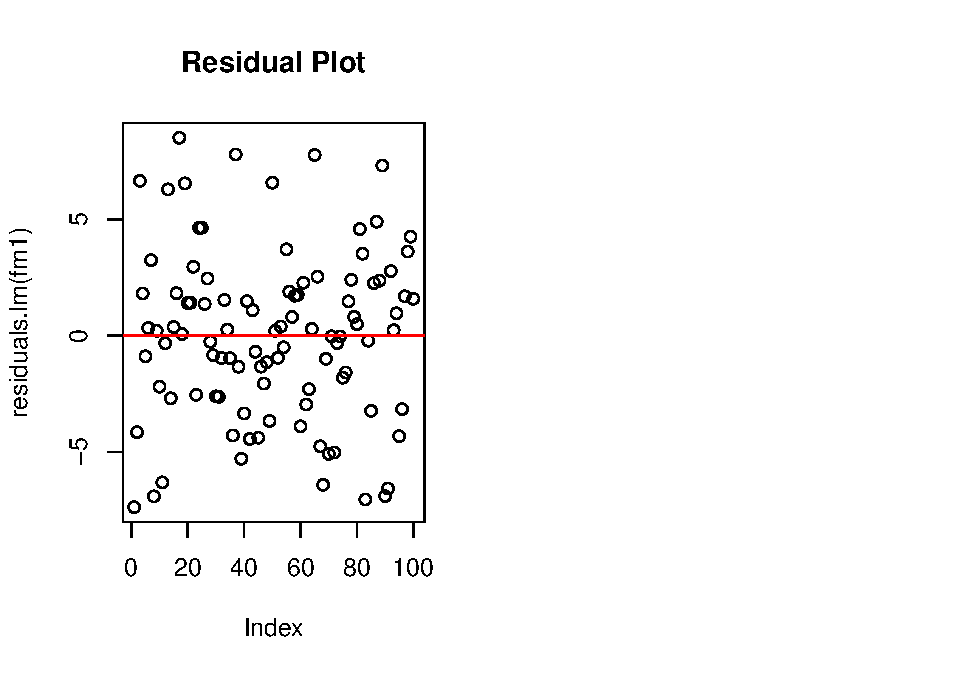
\includegraphics{MA_331_Final_-_Amane_and_Harry--2-_files/figure-latex/unnamed-chunk-2-1.pdf}

\begin{Shaded}
\begin{Highlighting}[]
\FunctionTok{qqnorm}\NormalTok{(}\FunctionTok{residuals}\NormalTok{(fm1),}\AttributeTok{main=}\StringTok{"QQ Plot"}\NormalTok{)}
\FunctionTok{abline}\NormalTok{(}\DecValTok{0}\NormalTok{,}\DecValTok{3}\NormalTok{, }\AttributeTok{col=}\StringTok{"red"}\NormalTok{)}
\end{Highlighting}
\end{Shaded}

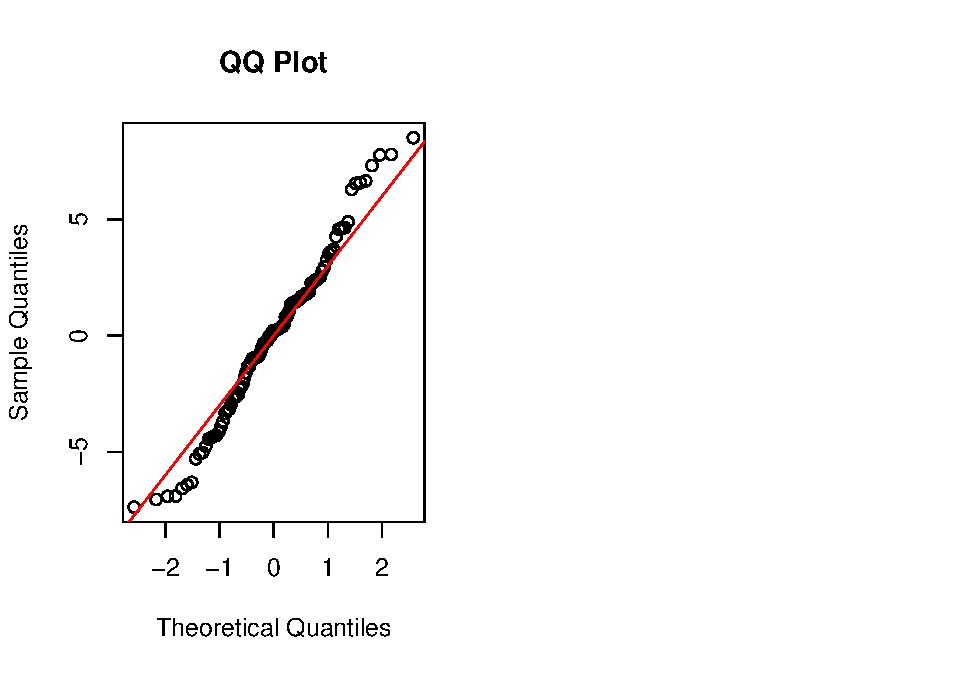
\includegraphics{MA_331_Final_-_Amane_and_Harry--2-_files/figure-latex/unnamed-chunk-2-2.pdf}

From the residual plot, it appears that the residuals are randomly
dispersed around the horizontal line at zero, which suggests that the
linear model may be appropriate. The normal Q-Q plot shows that the
residuals roughly follow a straight line, indicating that they are
approximately normally distributed. This supports the assumption of
normality in the linear regression model.Overall, the current regression
model seems to be a good fit for the data based on these diagnostics.

\hypertarget{problem-3}{%
\subsubsection{Problem 3}\label{problem-3}}

\begin{Shaded}
\begin{Highlighting}[]
\FunctionTok{kable}\NormalTok{(}\FunctionTok{coefficients}\NormalTok{(}\FunctionTok{summary}\NormalTok{(fm1)))}
\end{Highlighting}
\end{Shaded}

\begin{longtable}[]{@{}lrrrr@{}}
\toprule\noalign{}
& Estimate & Std. Error & t value &
Pr(\textgreater\textbar t\textbar) \\
\midrule\noalign{}
\endhead
\bottomrule\noalign{}
\endlastfoot
(Intercept) & 29.5782471 & 1.4119783 & 20.948089 & 0.0e+00 \\
PA & -0.6546858 & 0.1583361 & -4.134784 & 7.5e-05 \\
\end{longtable}

\begin{Shaded}
\begin{Highlighting}[]
\NormalTok{(}\FunctionTok{sigma}\NormalTok{(fm1))}\SpecialCharTok{\^{}}\DecValTok{2}
\end{Highlighting}
\end{Shaded}

\begin{verbatim}
## [1] 13.35817
\end{verbatim}

\begin{Shaded}
\begin{Highlighting}[]
\FunctionTok{cat}\NormalTok{(}\StringTok{"Regression Equation: BMI = 29.578 {-} 0.655 x PA"}\NormalTok{)}
\end{Highlighting}
\end{Shaded}

\begin{verbatim}
## Regression Equation: BMI = 29.578 - 0.655 x PA
\end{verbatim}

\begin{Shaded}
\begin{Highlighting}[]
\FunctionTok{plot}\NormalTok{(pabmi}\SpecialCharTok{$}\NormalTok{PA, pabmi}\SpecialCharTok{$}\NormalTok{BMI, }\AttributeTok{main =} \StringTok{"BMI vs PA"}\NormalTok{, }\AttributeTok{xlab =} \StringTok{"Physical Activity (PA)"}\NormalTok{, }\AttributeTok{ylab =} \StringTok{"Body Mass Index (BMI)"}\NormalTok{, }\AttributeTok{pch =} \DecValTok{19}\NormalTok{, }\AttributeTok{col =} \StringTok{"blue"}\NormalTok{)}
\FunctionTok{abline}\NormalTok{(fm1, }\AttributeTok{col =} \StringTok{"red"}\NormalTok{, }\AttributeTok{lwd =} \DecValTok{2}\NormalTok{)}
\end{Highlighting}
\end{Shaded}

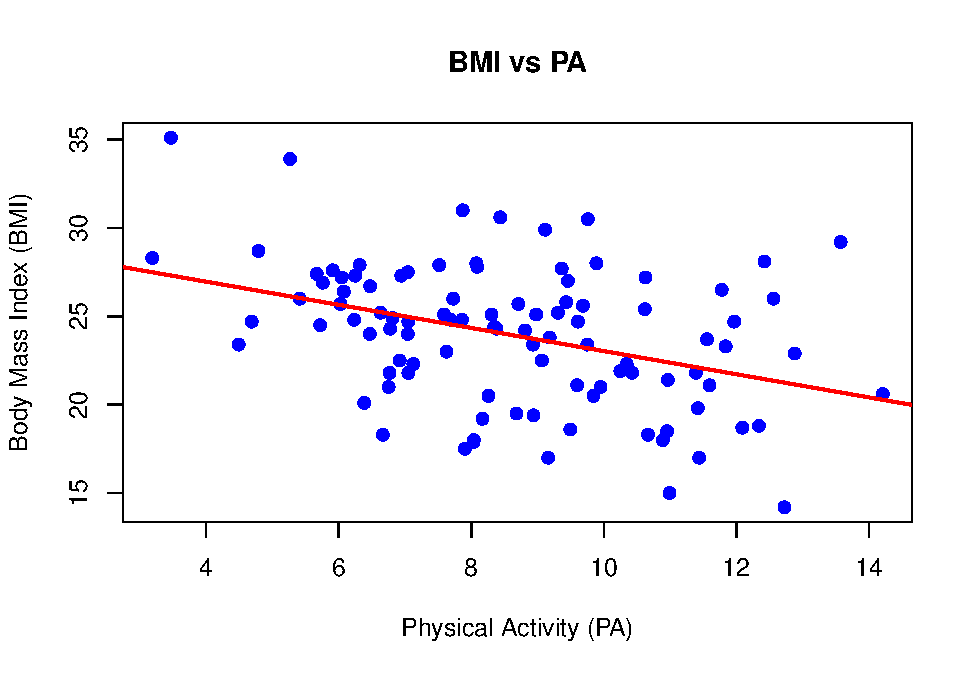
\includegraphics{MA_331_Final_-_Amane_and_Harry--2-_files/figure-latex/unnamed-chunk-3-1.pdf}

\hypertarget{problem-4}{%
\subsubsection{Problem 4}\label{problem-4}}

\begin{Shaded}
\begin{Highlighting}[]
\FunctionTok{kable}\NormalTok{(}\FunctionTok{anova}\NormalTok{(fm1))}
\end{Highlighting}
\end{Shaded}

\begin{longtable}[]{@{}lrrrrr@{}}
\toprule\noalign{}
& Df & Sum Sq & Mean Sq & F value & Pr(\textgreater F) \\
\midrule\noalign{}
\endhead
\bottomrule\noalign{}
\endlastfoot
PA & 1 & 228.3772 & 228.37719 & 17.09644 & 7.5e-05 \\
Residuals & 98 & 1309.1007 & 13.35817 & NA & NA \\
\end{longtable}

The hypothesis test for the slope parameter in the regression model of
BMI as a function of PA yields a p-value of 7.5e-05, which is
significantly less than the alpha level of 0.05. This indicates strong
statistical evidence to reject the null hypothesis that the slope is
zero. Therefore, we conclude that there is a significant negative
relationship between PA (Physical Activity) and BMI (Body Mass Index),
suggesting that increases in PA are associated with decreases in BMI.

\hypertarget{problem-5}{%
\subsubsection{Problem 5}\label{problem-5}}

\begin{Shaded}
\begin{Highlighting}[]
\FunctionTok{kable}\NormalTok{(}\FunctionTok{confint}\NormalTok{(fm1))}
\end{Highlighting}
\end{Shaded}

\begin{longtable}[]{@{}lrr@{}}
\toprule\noalign{}
& 2.5 \% & 97.5 \% \\
\midrule\noalign{}
\endhead
\bottomrule\noalign{}
\endlastfoot
(Intercept) & 26.7762222 & 32.3802721 \\
PA & -0.9688987 & -0.3404729 \\
\end{longtable}

The 95\% confidence interval is from (-0.97,-0.34)

\hypertarget{problem-6}{%
\subsubsection{Problem 6}\label{problem-6}}

\begin{Shaded}
\begin{Highlighting}[]
\FunctionTok{kable}\NormalTok{(}\FunctionTok{anova}\NormalTok{(fm1))}
\end{Highlighting}
\end{Shaded}

\begin{longtable}[]{@{}lrrrrr@{}}
\toprule\noalign{}
& Df & Sum Sq & Mean Sq & F value & Pr(\textgreater F) \\
\midrule\noalign{}
\endhead
\bottomrule\noalign{}
\endlastfoot
PA & 1 & 228.3772 & 228.37719 & 17.09644 & 7.5e-05 \\
Residuals & 98 & 1309.1007 & 13.35817 & NA & NA \\
\end{longtable}

T he Pr(\textgreater F) (p-value) is less than 0.05, you can reject the
null hypothesis that the model with no predictors fits the data as well
as your model. This means that the overall regression model is
statistically significant, and the predictor (PA) provides a better fit
to the data than the intercept-only model.

\hypertarget{problem-7}{%
\subsubsection{Problem 7}\label{problem-7}}

\begin{Shaded}
\begin{Highlighting}[]
\FunctionTok{summary}\NormalTok{(fm1)}
\end{Highlighting}
\end{Shaded}

\begin{verbatim}
## 
## Call:
## lm(formula = BMI ~ PA, data = pabmi)
## 
## Residuals:
##     Min      1Q  Median      3Q     Max 
## -7.3819 -2.5636  0.2062  1.9820  8.5078 
## 
## Coefficients:
##             Estimate Std. Error t value Pr(>|t|)    
## (Intercept)  29.5782     1.4120  20.948  < 2e-16 ***
## PA           -0.6547     0.1583  -4.135  7.5e-05 ***
## ---
## Signif. codes:  0 '***' 0.001 '**' 0.01 '*' 0.05 '.' 0.1 ' ' 1
## 
## Residual standard error: 3.655 on 98 degrees of freedom
## Multiple R-squared:  0.1485, Adjusted R-squared:  0.1399 
## F-statistic:  17.1 on 1 and 98 DF,  p-value: 7.503e-05
\end{verbatim}

\begin{Shaded}
\begin{Highlighting}[]
\NormalTok{SSM }\OtherTok{=} \FunctionTok{sum}\NormalTok{((}\FunctionTok{predict}\NormalTok{(fm1) }\SpecialCharTok{{-}} \FunctionTok{mean}\NormalTok{(pabmi}\SpecialCharTok{$}\NormalTok{BMI))}\SpecialCharTok{\^{}}\DecValTok{2}\NormalTok{) ; SSM}
\end{Highlighting}
\end{Shaded}

\begin{verbatim}
## [1] 228.3772
\end{verbatim}

\begin{Shaded}
\begin{Highlighting}[]
\NormalTok{SST }\OtherTok{=} \FunctionTok{sum}\NormalTok{((pabmi}\SpecialCharTok{$}\NormalTok{BMI }\SpecialCharTok{{-}} \FunctionTok{mean}\NormalTok{(pabmi}\SpecialCharTok{$}\NormalTok{BMI))}\SpecialCharTok{\^{}}\DecValTok{2}\NormalTok{); SST}
\end{Highlighting}
\end{Shaded}

\begin{verbatim}
## [1] 1537.478
\end{verbatim}

The coefficient of determination is 0.15. SSM is 228.38 and SST is
1537.48

\hypertarget{problem-8}{%
\subsubsection{Problem 8}\label{problem-8}}

\begin{Shaded}
\begin{Highlighting}[]
\NormalTok{observation }\OtherTok{=} \FunctionTok{data.frame}\NormalTok{(}\AttributeTok{PA =} \FloatTok{27.85}\NormalTok{)}

\FunctionTok{predict}\NormalTok{(fm1,}\AttributeTok{newdata=}\NormalTok{observation,}\AttributeTok{interval=}\StringTok{"confidence"}\NormalTok{,}\AttributeTok{level=}\FloatTok{0.95}\NormalTok{)}
\end{Highlighting}
\end{Shaded}

\begin{verbatim}
##        fit      lwr      upr
## 1 11.34525 5.257584 17.43291
\end{verbatim}

The predicted BMI for a PA of 27.85 is approximately 11.34525, with a
95\% confidence interval ranging from about 5.257584 to 17.43291. This
interval indicates where the true mean response is expected to fall with
95\% confidence, assuming the model is correct and the assumptions hold.

\hypertarget{problem-9}{%
\subsubsection{Problem 9}\label{problem-9}}

\begin{Shaded}
\begin{Highlighting}[]
\NormalTok{observation }\OtherTok{=} \FunctionTok{data.frame}\NormalTok{(}\AttributeTok{PA =} \FloatTok{31.25}\NormalTok{)}

\FunctionTok{predict}\NormalTok{(fm1,}\AttributeTok{newdata=}\NormalTok{observation,}\AttributeTok{interval=}\StringTok{"prediction"}\NormalTok{,}\AttributeTok{level=}\FloatTok{0.9}\NormalTok{)}
\end{Highlighting}
\end{Shaded}

\begin{verbatim}
##        fit      lwr      upr
## 1 9.119317 0.597295 17.64134
\end{verbatim}

The predicted BMI for a PA of 31.25 is approximately 9.119317, with a
90\% prediction interval ranging from about 0.597295 to 17.64134. This
interval indicates where the actual observed BMI is expected to fall
with 90\% confidence, assuming the model is correct and the assumptions
hold.{]}

\hypertarget{problem-10}{%
\subsubsection{Problem 10}\label{problem-10}}

\begin{Shaded}
\begin{Highlighting}[]
\NormalTok{fm2}\OtherTok{=} \FunctionTok{lm}\NormalTok{(BMI }\SpecialCharTok{\textasciitilde{}} \FunctionTok{poly}\NormalTok{(PA,}\DecValTok{2}\NormalTok{), }\AttributeTok{data=}\NormalTok{pabmi)}
\FunctionTok{summary}\NormalTok{(fm2)}
\end{Highlighting}
\end{Shaded}

\begin{verbatim}
## 
## Call:
## lm(formula = BMI ~ poly(PA, 2), data = pabmi)
## 
## Residuals:
##     Min      1Q  Median      3Q     Max 
## -8.1159 -2.3779  0.1315  2.2638  7.7518 
## 
## Coefficients:
##              Estimate Std. Error t value Pr(>|t|)    
## (Intercept)   23.9390     0.3612  66.285  < 2e-16 ***
## poly(PA, 2)1 -15.1122     3.6115  -4.184 6.28e-05 ***
## poly(PA, 2)2   6.6269     3.6115   1.835   0.0696 .  
## ---
## Signif. codes:  0 '***' 0.001 '**' 0.01 '*' 0.05 '.' 0.1 ' ' 1
## 
## Residual standard error: 3.612 on 97 degrees of freedom
## Multiple R-squared:  0.1771, Adjusted R-squared:  0.1601 
## F-statistic: 10.44 on 2 and 97 DF,  p-value: 7.838e-05
\end{verbatim}

The regression polynomial equation is Y = 23.94 − 15.11x + 6.63x. If the
adjusted for the polynomial model is higher than that for the linear
model, the polynomial model is better. This indicates that including the
squared term of PA provides a better fit to the data, capturing more of
the variability in BMI. The reason a model with a higher adjusted R\^{}2
is considered better is that it explains a greater proportion of the
variance in the dependent variable, after adjusting for the number of
predictors in the model, thus potentially capturing more complex
relationships between the variables.

\hypertarget{problem-11}{%
\subsubsection{Problem 11}\label{problem-11}}

\begin{Shaded}
\begin{Highlighting}[]
\FunctionTok{plot}\NormalTok{(BMI }\SpecialCharTok{\textasciitilde{}}\NormalTok{ PA, }\AttributeTok{data=}\NormalTok{pabmi, }\AttributeTok{main=}\StringTok{"Simple linear regression and polynomial regression models"}\NormalTok{)}
\FunctionTok{abline}\NormalTok{(fm1, }\AttributeTok{col=}\StringTok{"green"}\NormalTok{,}\AttributeTok{lwd=}\DecValTok{3}\NormalTok{)}
\NormalTok{pavals }\OtherTok{\textless{}{-}} \FunctionTok{seq}\NormalTok{(}\FunctionTok{min}\NormalTok{(pabmi}\SpecialCharTok{$}\NormalTok{PA), }\FunctionTok{max}\NormalTok{(pabmi}\SpecialCharTok{$}\NormalTok{PA), }\AttributeTok{length.out =} \DecValTok{100}\NormalTok{)}
\FunctionTok{lines}\NormalTok{(pavals, }\FunctionTok{predict}\NormalTok{(fm2, }\AttributeTok{newdata =} \FunctionTok{data.frame}\NormalTok{(}\AttributeTok{PA =}\NormalTok{ pavals)),}\AttributeTok{col=}\StringTok{"red"}\NormalTok{,}\AttributeTok{lwd=}\DecValTok{3}\NormalTok{)}
\FunctionTok{legend}\NormalTok{(}\StringTok{"bottomright"}\NormalTok{,}\FunctionTok{c}\NormalTok{(}\StringTok{"PA"}\NormalTok{, }\StringTok{"Poly PA"}\NormalTok{), }\AttributeTok{col=}\FunctionTok{c}\NormalTok{(}\StringTok{"green"}\NormalTok{,}\StringTok{"red"}\NormalTok{),}\AttributeTok{lwd=}\DecValTok{3}\NormalTok{)}
\end{Highlighting}
\end{Shaded}

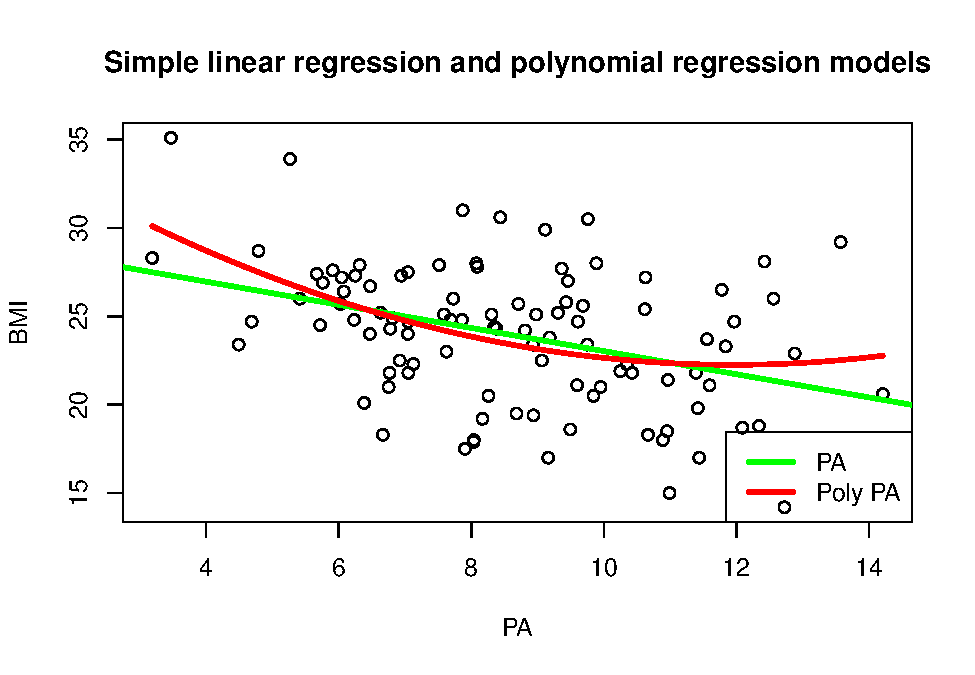
\includegraphics{MA_331_Final_-_Amane_and_Harry--2-_files/figure-latex/unnamed-chunk-11-1.pdf}

\hypertarget{problem-12}{%
\subsubsection{Problem 12}\label{problem-12}}

\[
Y = X \beta + \epsilon
\]

\[
Y = \begin{bmatrix}
    y_1 \\
    y_2 \\
    \vdots \\
    y_n
\end{bmatrix} \quad
X = \begin{bmatrix}
    1 & (x_1 - \bar{x}) \\
    1 & (x_2 - \bar{x}) \\
    \vdots & \vdots \\
    1 & (x_n - \bar{x})
\end{bmatrix} \quad
\beta = \begin{bmatrix}
    \beta_0 \\
    \beta_1
\end{bmatrix} \quad
\epsilon = \begin{bmatrix}
    \epsilon_1 \\
    \epsilon_2 \\
    \vdots \\
    \epsilon_n
\end{bmatrix}
\]

\hfill\break

\hypertarget{problem-13}{%
\subsubsection{Problem 13}\label{problem-13}}

\[
X = \begin{bmatrix}
1 & (x_1 - \bar{x}) \\
1 & (x_2 - \bar{x}) \\
\vdots & \vdots \\
1 & (x_n - \bar{x})
\end{bmatrix} \quad
Y = \begin{bmatrix}
y_1 \\
y_2 \\
\vdots \\
y_n
\end{bmatrix}
\]

\[
X' = \begin{bmatrix}
1 & 1 & \dots & 1 \\
(x_1 - \bar{x}) & (x_2 - \bar{x}) & \dots & (x_n - \bar{x})
\end{bmatrix}
\]

\[
X'X = \begin{bmatrix}
n & \sum (x_i - \bar{x}) \\
\sum (x_i - \bar{x}) & \sum (x_i - \bar{x})^2
\end{bmatrix} = \begin{bmatrix}
n & 0 \\
0 & \sum (x_i - \bar{x})^2
\end{bmatrix}
\]

\[
(X'X)^{-1} = \begin{bmatrix}
\frac{1}{n} & 0 \\
0 & \frac{1}{\sum (x_i - \bar{x})^2}
\end{bmatrix}
\]

\[
X'Y = \begin{bmatrix}
\sum y_i \\
\sum ((x_i - \bar{x})y_i)
\end{bmatrix}
\]

\[
\hat{\beta} = (X'X)^{-1} X'Y = \begin{bmatrix}
\frac{\sum y_i}{n} \\
\frac{\sum ((x_i - \bar{x})y_i)}{\sum (x_i - \bar{x})^2}
\end{bmatrix}
\]

\end{document}
